% Springer Nature journal article template, version 3.1 (December 2024)
\documentclass[pdflatex,sn-mathphys-num]{sn-jnl}
\usepackage{graphicx}
\usepackage{multirow}
\usepackage{amsmath,amssymb,amsfonts}
\usepackage{booktabs}
\usepackage{siunitx}
\usepackage{cleveref}
\usepackage{xcolor}
\raggedbottom

\begin{document}

\title[ShiftGuard for robust traffic forecasting]{ShiftGuard: Risk-Controlled Spatiotemporal Traffic Forecasting under Compound Regime Shifts and Sensor Outages}

\author[1]{\fnm{Shishir Singh} \sur{Chauhan}}

\affil[1]{\orgname{Manipal University Jaipur},
\orgaddress{\street{Dehmi Kalan, Jaipur-Ajmer Expressway},
\city{Jaipur}, \postcode{303007}, \state{Rajasthan}, \country{India}}}

\abstract{Accurate short-term traffic forecasting is essential for intelligent transportation systems, but conventional benchmarks largely assume stable traffic regimes and fully observed sensor networks. This study presents ShiftGuard, a risk-controlled spatiotemporal framework for compound shifts in traffic conditions and sensor availability. ShiftGuard jointly produces point forecasts, calibrated node--horizon prediction intervals, and origin-level abstention decisions using reliability-conditioned graph--temporal encoding, structured-outage augmentation, probabilistic scale estimation, and prequential group-adaptive conformal calibration. A leakage-controlled protocol evaluates independent, burst, contiguous-region, and hub outages at multiple severities on METR-LA and PEMS-BAY. Across 640 confirmatory stress runs over five seeds, ShiftGuard reduces mean absolute error relative to the strongest locally reproduced transformer from 3.74 to 3.40 mph on METR-LA and from 2.49 to 1.94 mph on PEMS-BAY. At 30\% outage severity, risk control retains 86\% and 98\% of forecast origins while limiting empirical origin-level failure to 8\% and 2\%, respectively. Although clean PEMS-BAY accuracy remains 0.027 mph behind STAEformer, the results show that ShiftGuard provides stronger robustness, calibrated uncertainty, and actionable failure control under compound shifts.}

\keywords{traffic forecasting , intelligent transportation systems , spatiotemporal graph neural network , sensor outage , distribution shift , conformal prediction , selective prediction}

\maketitle

\section{Introduction}
Short-term network traffic forecasting is a core perception service in an
intelligent transportation system (ITS). Forecasts of speed, flow, and
occupancy support route guidance, ramp metering, signal coordination,
congestion warning, incident management, emergency response, and the timing of
traveler-information messages. A useful forecast must therefore do more than
minimize an offline average: it must arrive within an operational latency
budget, remain usable when field sensors fail, and expose enough uncertainty
for a downstream controller to decide whether intervention is warranted.
METR-LA and PEMS-BAY have enabled reproducible progress on this problem by
representing a freeway system as multivariate time series attached to a sensor
graph~\cite{li2018dcrnn}. They remain the most common common-denominator
benchmarks for comparing graph-based forecasting methods, despite their age
and highway-centric scope.

The dominant modeling trajectory has been to improve spatiotemporal feature
extraction. DCRNN models directed traffic diffusion inside a recurrent
encoder--decoder~\cite{li2018dcrnn}; STGCN couples spectral graph operations
with gated temporal convolutions~\cite{yu2018stgcn}; and Graph WaveNet learns an
adaptive adjacency together with dilated temporal filters
~\cite{wu2019graphwavenet}. Later systems learn node-specific parameters
~\cite{bai2020agcrn}, discrete or dynamic graphs
~\cite{shang2021gts,shao2022d2stgnn}, synchronous spatiotemporal neighborhoods
~\cite{song2020stsgcn}, propagation delays~\cite{jiang2023pdformer}, or
memory-conditioned meta-graphs~\cite{jiang2023megacrn}. Attention and
transformer designs extend the receptive field
~\cite{zheng2020gman,lan2022dstagnn,liu2023staeformer}, whereas STID and FC-GAGA
show that simple identity embeddings or fully connected gated blocks can be
surprisingly competitive~\cite{shao2022stid,oreshkin2021fcgaga}. The lesson is
important for credible novelty: additional architectural complexity is not, by
itself, evidence of a better deployable forecaster.

Most benchmark tables nevertheless assume that the input graph is fully
observed and that the test distribution is represented by a single clean
chronological block. This assumption is fragile in practice. Loop detectors
and roadside units may be unavailable because of communication loss,
maintenance, power interruption, calibration drift, or shared infrastructure
failure. Such missingness is rarely independent. A communications outage can
remove a contiguous corridor; a gateway failure can remove high-centrality
sensors; and intermittent hardware can create temporal bursts. At the same
time, traffic can move from free flow to congestion, recover after an incident,
or exhibit volatility not represented in training. Graph message passing can
amplify these failures because a corrupted or absent node influences its
neighbors. Work on tensor completion and graph-tensor imputation demonstrates
that topology helps recover missing network observations
~\cite{baggag2021tensor,xu2023graphtensor}, while masked pretraining improves
representation learning~\cite{sun2023stmae,gao2024stdmae}. Yet imputation
accuracy or independent random masking does not answer how a forecaster behaves
under simultaneous regime shift and spatially correlated outage.

Average point error is also an incomplete operational signal. A low test MAE
can coexist with large errors during a congestion transition or at a small set
of safety-critical sensors. Likewise, 90\% marginal prediction-interval
coverage can hide serious undercoverage at particular nodes, horizons, or
traffic regimes. Deep ensembles and probabilistic spatiotemporal models expose
aleatoric or epistemic variation~\cite{wu2021uq,liu2024ensembleuq}, and
conformal prediction can wrap a black-box forecaster with frequentist
intervals under stated assumptions~\cite{stankeviciute2021conformal}. Online
conformal methods respond to changing distributions
~\cite{gibbs2024online,angelopoulos2024online}. However, an interval alone does
not tell an ITS whether a complete 12-step network forecast should be acted on.
Selective prediction provides the missing decision layer: the system may
retain a forecast when its estimated risk is acceptable and abstain when it is
not. That choice is naturally evaluated through retained coverage,
risk--coverage curves, and the failure rate among accepted forecasts, not only
through interval width.

These observations motivate the joint question studied here: \emph{when both
the traffic regime and sensor-availability process differ from training, can a
computationally compact forecaster deliver accurate point predictions,
well-calibrated node--horizon intervals, and a leakage-free forecast-origin
decision to act or abstain?} The question is deliberately stricter than robust
point forecasting. It treats the output consumed by an ITS as one network-wide
forecast tensor, acknowledges dependence among its node--horizon cells, and
requires calibration and threshold selection to use only information available
before the current target resolves. Recent traffic conformal approaches adapt
intervals to topology or volatility~\cite{patil2024conformal,wang2026csth}, and
recent missing-sensor methods address cold-start or reliability-aware graph
construction~\cite{wang2026scsamg,wu2026cast}. Our 36-study evidence audit found
no prior method that jointly benchmarks point prediction, subgroup interval
reliability, and origin-level abstention across independent, temporal-burst,
contiguous-region, and high-centrality outages on both METR-LA and PEMS-BAY.

We address the gap with ShiftGuard. Its forecasting component concatenates
speed and observation masks, learns a lightweight temporal representation, and
combines static and adaptive spatial propagation. Training applies a curriculum
of structured outages so that the model must use partial histories rather than
learn only the clean sensor manifold. A probabilistic head supplies
heterogeneity-aware scales. At deployment, node--horizon nonconformity scores
are updated prequentially from resolved past origins, and interval width ranks
whole forecast tensors. A disjoint construction/certification split among past
origins prevents the selective threshold from being chosen and evaluated on
the same outcomes. We do not claim a distribution-free guarantee under
arbitrary temporal dependence; empirical prequential reliability and the
assumptions of the binomial certificate are reported separately.

The experimental motivation is equally important. Clean accuracy alone would
lead to an incorrect conclusion: ShiftGuard is statistically tied with the
local STAEformer on METR-LA and is 0.027 mph worse on clean PEMS-BAY. Under the
registered compound-shift protocol, however, the ordering changes. Across four
outage families, five severities, two datasets, and five seeds, ShiftGuard
reduces mean MAE relative to STAEformer by 0.347 mph on METR-LA and 0.546 mph on
PEMS-BAY. At 30\% severity it retains 86\% and 98\% of forecast origins while
limiting empirical accepted-origin failure to 8\% and 2\%. It also uses about
7--14 times fewer parameters than STAEformer, depending on the dataset. These
results position the work as a robustness and decision-reliability
contribution, not as a universal clean-data state of the art.

This work makes four contributions:
\begin{enumerate}
  \item We formulate traffic forecasting under compound temporal and
  measurement shift as a joint point, interval, and selective-decision task,
  and release a leakage-controlled protocol crossing traffic regimes with four
  graph-aware sensor-outage families and five severities.
  \item We develop a compact mask-aware graph--temporal forecaster trained by
  structured-outage augmentation and coupled to heterogeneity-aware
  probabilistic scale estimation.
  \item We introduce prequential node--horizon conformalization and an
  origin-level risk controller whose construction and certification samples
  are disjoint; reliability is evaluated using marginal and worst-group
  coverage, AURC, retention, and accepted-origin failure.
  \item We provide a five-seed, 640-run comparison against classical, recurrent,
  graph-convolutional, adaptive-graph, identity-based, and transformer
  baselines, together with ablations, hierarchical paired inference, runtime,
  memory, and parameter analyses. Negative ablations are used to narrow rather
  than inflate the novelty claim.
\end{enumerate}

The remainder of the article is organized as follows. Section~2 synthesizes
deterministic graph forecasting, shift and missing-data robustness,
probabilistic calibration, and selective prediction, and converts the survey
into an explicit gap analysis. Section~3 formulates the compound-shift task.
Section~4 presents the complete ShiftGuard architecture, learning objective,
calibration procedure, and decision rule. Section~5 describes the datasets,
splits, baselines, outage generators, metrics, and statistical protocol.
Section~6 reports clean accuracy, comparison charts, robustness, calibration,
ablation, and efficiency. Sections~7--9 discuss the evidence, limitations,
future work, and conclusions.

\section{Literature survey and gap analysis}
\subsection{From recurrent diffusion to adaptive graph learning}
Early deep traffic forecasting established the now-standard decomposition into
temporal dynamics and spatial interaction. DCRNN embeds a random-walk diffusion
operator in a sequence-to-sequence recurrent architecture, reflecting the
directed propagation of road conditions~\cite{li2018dcrnn}. STGCN replaces
recurrence with graph and gated temporal convolutions for efficient parallel
training~\cite{yu2018stgcn}. Graph WaveNet learns a latent adjacency and uses
dilated causal convolutions, demonstrating that data-driven connectivity can
complement or replace a distance graph~\cite{wu2019graphwavenet}. These methods
remain indispensable controls because many later gains depend on preprocessing,
split conventions, and implementation details as much as on the proposed
operator.

Subsequent work increases spatial adaptivity and heterogeneity. AGCRN generates
node-specific parameters from learned embeddings~\cite{bai2020agcrn}; GTS
learns a discrete graph jointly with prediction~\cite{shang2021gts}; and MTGNN
learns directed relations among variables without requiring a fixed road
graph~\cite{wu2020mtgnn}. STSGCN constructs localized synchronous
spatiotemporal graphs rather than treating space and time as sequentially
separable~\cite{song2020stsgcn}. FC-GAGA uses fully connected graph gates and
emphasizes computational efficiency~\cite{oreshkin2021fcgaga}. D2STGNN
decomposes traffic into inherent and diffusion signals while learning a dynamic
graph~\cite{shao2022d2stgnn}; MegaCRN retrieves meta-graph information from a
memory bank~\cite{jiang2023megacrn}; and PDFormer represents delayed propagation
and long-range spatial dependence~\cite{jiang2023pdformer}. DSTAGNN similarly
uses dynamic spatial-temporal awareness to model time-varying relations
~\cite{lan2022dstagnn}. These advances improve representation power, but the
observation mask is generally not an operational output and structured sensor
failure is not the primary evaluation axis.

Attention-based architectures extend this progression. GMAN uses transform
attention between encoded history and prediction horizons
~\cite{zheng2020gman}. STAEformer shows that vanilla self-attention becomes a
strong traffic forecaster when equipped with adaptive spatiotemporal embeddings
~\cite{liu2023staeformer}. Weaver factorizes full spatiotemporal attention by a
Kronecker approximation and introduces signed valence relationships
~\cite{cheong2026weaver}. In parallel, STID demonstrates that spatial identity
and temporal index embeddings can compete with substantially more complicated
graph models~\cite{shao2022stid}. The critical benchmark audit of Martin et al.
further reports that carefully trained spatially unaware models are stronger
than many published comparisons imply~\cite{martin2026audit}. Consequently, our
baseline suite includes persistence, ridge, linear, MLP, GRU, STGCN, DCRNN,
Graph WaveNet, AGCRN, STID, and STAEformer under one pipeline, and parameter and
latency measurements accompany error metrics.

\subsection{Long context, pretraining, routing, and nonstationarity}
Several approaches seek longer context or reusable representations rather than
ever deeper graph stacks. STEP pretrains a scalable temporal encoder on long
histories and supplies segment representations to a downstream STGNN
~\cite{shao2022step}. STMAE masks graph-aware spatial tokens and temporal
patches~\cite{sun2023stmae}; STD-MAE decouples spatial and temporal masked
reconstruction~\cite{gao2024stdmae}. These methods show that masking is a useful
learning signal, but their objective is representation quality on the natural
data distribution. ShiftGuard instead treats masks as explicit observations
and generates failures whose spatial and temporal geometry matches deployment
hazards.

Mixture and adaptation models address heterogeneity across contexts. TESTAM
routes recurring and non-recurring conditions among specialized spatial
experts~\cite{lee2024testam}. CompFormer retrieves analogous historical
representations at test time to compensate extreme traffic patterns
~\cite{zhang2023compformer}. Expand-and-Compress uses prompt pools for continual
spatiotemporal forecasting as streams and sensor networks evolve
~\cite{chen2025eac}. CAST-GNN learns causal invariances and dynamic associations
to generalize from observed weekdays to unseen contexts~\cite{wu2026cast}.
These studies demonstrate that nonstationarity cannot be dismissed as random
noise. Nevertheless, adapting a point predictor does not establish calibrated
subgroup uncertainty, and online parameter tuning is conceptually different
from deciding that a forecast tensor is unsafe to consume.

\subsection{Missing observations, outages, and graph reliability}
Missing traffic data has a long history in matrix and tensor completion.
Regularized tensor factorization jointly imputes missing road states and learns
latent temporal factors~\cite{baggag2021tensor}. Graph-tensor neural networks
unfold topology-aware completion algorithms for efficient network-wide
imputation~\cite{xu2023graphtensor}. Heterogeneous graph models and
availability-aware propagation likewise show that missing indicators should not
be confused with genuine zero traffic. These approaches usually optimize
reconstruction first, or couple imputation and forecasting under random missing
ratios. A forecast model can therefore score well even if it has not been
exposed to complete corridor or hub failures.

The distinction among failure geometries matters. Independent point loss tests
local redundancy. A temporal burst tests whether the model can extrapolate when
a sensor is silent for consecutive steps. A contiguous-region outage removes a
spatial cluster and therefore challenges neighborhood aggregation. A hub outage
targets sensors with high graph degree and can disproportionately interrupt
message flow. SC-SAMG studies cold-start forecasting for unseen sensors through
support-set adaptation~\cite{wang2026scsamg}, while recent reliability-oriented
graphs incorporate sensor confidence or physical constraints. However,
cold-start adaptation presumes a different information pattern from a sudden
deployment outage, and a reliability weight is not itself evidence of robust
decision quality. Our protocol therefore shares identical saved masks across
models and crosses each failure geometry with pre-defined traffic regimes.

\subsection{Probabilistic traffic forecasting and conformal calibration}
Probabilistic forecasting supplements a conditional center with an estimate of
dispersion or a predictive distribution. Bayesian graph neural networks,
quantile regression, heteroscedastic likelihoods, and deep ensembles represent
different combinations of aleatoric and epistemic uncertainty. A systematic
study by Wu et al. compares Bayesian and frequentist spatiotemporal uncertainty
routes~\cite{wu2021uq}; a later deep-ensemble framework combines simultaneous
quantile regression with ensemble diversity~\cite{liu2024ensembleuq}. These
methods are informative but may be miscalibrated when their likelihood family
or test distribution is misspecified.

Conformal prediction is attractive because it calibrates residual scores around
an arbitrary base predictor. Conformal time-series forecasting extends the
inductive framework to multi-horizon outputs under exchangeability conditions
~\cite{stankeviciute2021conformal}. Gibbs and Cand\`es address online prediction
under arbitrary distribution shifts through locally adaptive updates
~\cite{gibbs2024online}, while decaying-step online conformal prediction
improves behavior when a stable population quantile exists
~\cite{angelopoulos2024online}. CAP studies false-coverage-rate control after
adaptive selection~\cite{bao2025cap}. These theoretical distinctions are
essential: retrospective average coverage for an arbitrary sequence, marginal
coverage under exchangeability, and prospective conditional coverage are not
interchangeable claims.

Traffic-specific conformal models have begun to encode topology and volatility.
Patil et al. combine availability-aware graph construction with adaptive
intervals~\cite{patil2024conformal}. CSTH conditions interval scales on
hypergraph density and traffic volatility and evaluates blocked-time
calibration on METR-LA and PEMS-BAY~\cite{wang2026csth}. A regime-dependent
audit shows that aggregate interval coverage can conceal transition failures
~\cite{wang2026regime}. This motivates our node--horizon and regime reporting.
The remaining gap is operational: none of these systems jointly evaluates
structured graph outages and a risk-certified option to withhold an entire
network forecast.

\subsection{Selective prediction and operational decision making}
Selective prediction couples a predictor with a selection function. Instead of
forcing a low-confidence output into a controller, the system trades coverage
for lower conditional risk. In traffic forecasting this trade-off must be
defined carefully because one forecast origin contains hundreds or thousands
of correlated node--horizon cells. Treating every cell as an independent trial
would produce spuriously large calibration samples and unrealistically tight
certificates. We therefore define operational failure using the mean absolute
error of the complete forecast tensor and use its mean interval width as the
selection score. The threshold is constructed and certified on disjoint past
origins. CAP provides related theory for adaptively selected conformal outputs
~\cite{bao2025cap}, but graph outages and network-wide forecast decisions are
outside its application setting.

\begin{table*}[t]
\centering
\caption{Taxonomy of representative literature and the unresolved joint task.
``Struct.'' denotes explicitly structured sensor outages; ``groups'' denotes
node, horizon, or regime reliability; and ``abstain'' denotes an operational
selection decision rather than an interval alone.}
\label{tab:literature-taxonomy}
\scriptsize
\resizebox{\textwidth}{!}{%
\begin{tabular}{lllllll}
\toprule
Research line & Representative methods & Point forecast & Shift adaptation & Struct. outage & UQ/groups & Abstain \\
\midrule
Diffusion/convolution & DCRNN, STGCN, Graph WaveNet & yes & no & no & no & no \\
Adaptive graph & AGCRN, GTS, D2STGNN, MegaCRN & yes & partial & no & no & no \\
Attention/transformer & GMAN, PDFormer, STAEformer, Weaver & yes & partial & no & no & no \\
Simple/efficient & STID, FC-GAGA & yes & no & no & no & no \\
Pretraining & STEP, STMAE, STD-MAE & yes & partial & masking proxy & no & no \\
Extreme/continual & CompFormer, Expand--Compress, CAST-GNN & yes & yes & no & no & no \\
Imputation & tensor factorization, graph-tensor networks & indirect & no & partial & no & no \\
Probabilistic traffic & Bayesian/ensemble STGNNs & yes & no & no & intervals/no & no \\
Conformal traffic & availability-aware CP, CSTH & yes & yes & limited & intervals/partial & no \\
Selective inference & CAP, online conformal prediction & generic & yes & no & generic & yes \\
\midrule
ShiftGuard protocol & structured augmentation + prequential risk control & yes & yes & four families & intervals/groups & yes \\
\bottomrule
\end{tabular}}
\end{table*}

\subsection{Benchmarking practice and reproducibility}
Traffic-forecasting comparisons are unusually sensitive to protocol choices.
Published METR-LA and PEMS-BAY tables may differ in the raw-file revision,
interpretation of zero values, chronological boundary, scaler fitting,
horizon-wise aggregation, treatment of missing targets, and whether validation
or test data influence graph construction. A model can also be reported from
its best seed while another is averaged over seeds. The critical audit of
Martin et al. demonstrates that these details can reverse conclusions about
the value of spatial modeling~\cite{martin2026audit}. Consequently,
literature-reported numbers are useful for historical context but are not
exchangeable with results from a new local pipeline.

Robustness evaluation introduces further degrees of freedom. Random masks must
be shared across models; otherwise a method may receive an easier failed-sensor
set. Severity may refer to cells, nodes, or complete temporal windows, which
produce qualitatively different information loss. Calibration can be static,
rolling, global, or group-specific. If a test residual helps select its own
interval quantile or abstention threshold, apparent reliability is optimistic.
Finally, reporting only the average across outage families can hide a method
that fails catastrophically on a contiguous region or central hub. These
concerns motivate our saved-mask design, family-wise artifacts, chronological
prequential updates, and explicit separation of threshold construction from
certification.

Efficiency is also part of reproducibility. Transformer accuracy may require a
parameter, memory, and latency budget that is unavailable at a traffic control
center or roadside device, while lightweight identity models can provide a
stronger practical reference~\cite{shao2022stid,liu2023staeformer}. Parameter
count alone is insufficient because recurrent sequential operations, dense
attention, and graph kernels have different runtime behavior. We therefore
measure profiler-observed operations, batch-one latency, batch-eight
throughput, and peak allocated GPU memory on one disclosed platform. These
measurements are not universal hardware rankings, but they make the local
accuracy--reliability trade-off auditable.

Taken together, reproducibility requires more than releasing model code. It
requires freezing data transforms, saving generated failures, distinguishing
local reproductions from external numbers, retaining all confirmatory seeds,
and regenerating tables from structured outputs. The present study treats this
evaluation system as part of the contribution because a claim about reliable
forecasting cannot be stronger than the protocol used to produce it.

\subsection{Gap synthesis and research questions}
Table~\ref{tab:literature-taxonomy} reveals four gaps. First, deterministic
traffic forecasting and missing-data reconstruction are usually evaluated as
separate tasks, leaving compound regime--outage shift under-specified. Second,
probabilistic and conformal studies emphasize marginal coverage, which can hide
unreliable nodes, horizons, and transition regimes. Third, few traffic systems
convert uncertainty into an origin-level act/abstain decision with explicit
risk and retention metrics. Fourth, complexity can obscure the true cause of
improvement unless simple baselines, efficiency, and negative ablations are
reported. We consequently ask: (RQ1) Does structured-outage training improve
point robustness across both benchmarks and all four outage geometries? (RQ2)
Does prequential group calibration improve worst-group reliability under
drift? (RQ3) Can origin-level selection reduce accepted-forecast failure while
retaining useful coverage? (RQ4) Which architectural or training components
actually explain the gains, and what computational cost do they impose?

\section{Problem formulation}
\subsection{Traffic network, observations, and prediction target}
Let $\mathcal{G}=(\mathcal{V},\mathcal{E},A)$ denote a directed traffic-sensor
network, where $\mathcal{V}=\{v_1,\ldots,v_N\}$ is the sensor set,
$\mathcal{E}$ contains spatial relations, and $A\in\mathbb{R}_{+}^{N\times N}$
is a weighted adjacency matrix. An edge weight may encode road-network
proximity or empirical dependence between two sensors. Let
$Z_t\in\mathbb{R}^{N}$ be the conceptually complete vector of traffic speeds at
five-minute instant $t$. Because measurements can be naturally absent or
deliberately removed by a stress scenario, the model observes
\begin{equation}
 X_t=M_t\odot Z_t, \qquad M_t\in\{0,1\}^{N},
 \label{eq:masked-observation}
\end{equation}
where $M_{t,i}=1$ means that the speed at sensor $i$ is available. In the
implementation, masking is applied after standardization and the binary
indicator is passed to the model; hence a missing value is distinguishable
from a genuine zero-speed observation.

A forecast origin $t$ uses a history of $P=12$ observations, corresponding to
the preceding 60 minutes,
\begin{equation}
 \mathbf{X}_t=[X_{t-P+1},\ldots,X_t]\in\mathbb{R}^{P\times N},\qquad
 \mathbf{M}_t=[M_{t-P+1},\ldots,M_t]\in\{0,1\}^{P\times N},
\end{equation}
together with calendar covariates $C_t$ and graph $\mathcal{G}$. The target is
the next $H=12$ speed vectors,
\begin{equation}
 \mathbf{Y}_t=[Z_{t+1},\ldots,Z_{t+H}]\in\mathbb{R}^{H\times N}.
 \label{eq:forecast-target}
\end{equation}
Any intrinsically unavailable target cell is excluded by a target-validity
mask $O_t\in\{0,1\}^{H\times N}$. A forecasting system is therefore a mapping
\begin{equation}
 f_{\theta}:(\mathbf{X}_t,\mathbf{M}_t,C_t,\mathcal{G})
 \longmapsto (\widehat{\mathbf{Y}}_t,\mathbf{S}_t),
 \label{eq:probabilistic-forecast-map}
\end{equation}
where $\widehat{\mathbf{Y}}_t$ is the point-forecast tensor and
$\mathbf{S}_t>0$ is a learned uncertainty scale for every horizon--sensor
cell.

\subsection{Compound regime and sensor-availability shift}
Let $e_t\in\mathcal{E}_{\mathrm{env}}$ describe the traffic environment at
origin $t$, including recurrent congestion, free flow, transition periods, and
atypical demand. The joint data-generating distribution is written as
\begin{equation}
 (\mathbf{X}_t,\mathbf{M}_t,\mathbf{Y}_t,C_t)\sim
 \mathcal{P}_{e_t}.
\end{equation}
Standard empirical-risk minimization implicitly expects future origins to
resemble the training mixture $\mathcal{P}_{\mathrm{tr}}$. The deployment
setting considered here permits both the traffic mechanism and the observation
mechanism to change:
\begin{equation}
 \mathcal{P}_{\mathrm{te}}(\mathbf{Y}_t\mid\mathbf{X}_t,C_t,\mathcal{G})
 \ne \mathcal{P}_{\mathrm{tr}}(\mathbf{Y}_t\mid\mathbf{X}_t,C_t,\mathcal{G}),
 \quad
 \mathcal{P}_{\mathrm{te}}(\mathbf{M}_t\mid e_t,\mathcal{G})
 \ne \mathcal{P}_{\mathrm{tr}}(\mathbf{M}_t\mid e_t,\mathcal{G}).
 \label{eq:compound-shift}
\end{equation}
The first inequality represents regime shift; the second represents sensor
outage shift. Their concurrence is a \emph{compound shift}. Missingness is not
assumed to be independent and identically distributed. Instead, an outage
operator $\mathcal{T}_{\omega,s}$ transforms the intrinsic mask according to
family $\omega$ and severity $s$:
\begin{equation}
 \widetilde{\mathbf{M}}_t=
 \mathcal{T}_{\omega,s}(\mathbf{M}_t;\mathcal{G}),
 \qquad
 \omega\in\{\text{independent, burst, region, hub}\}.
 \label{eq:outage-operator}
\end{equation}
Independent outages remove sensor--time cells, bursts remove temporally
contiguous suffixes, region outages remove connected subgraphs, and hub outages
remove high-centrality sensors. Thus the shift may destroy precisely the
neighbors on which a graph forecaster relies. Severity $s\in[0,1]$ controls the
requested fraction of unavailable observations, subject to the geometry of the
selected family.

\subsection{Point and probabilistic forecasting objectives}
For a single origin, masked mean absolute error is
\begin{equation}
 \ell_{\mathrm{MAE}}(t)=
 \frac{\sum_{h=1}^{H}\sum_{i=1}^{N}O_{t,h,i}
 |Y_{t,h,i}-\widehat{Y}_{t,h,i}|}
 {\sum_{h=1}^{H}\sum_{i=1}^{N}O_{t,h,i}}.
 \label{eq:origin-mae}
\end{equation}
The first objective is to minimize expected point risk not only for clean
origins but across an explicit set $\mathcal{Q}$ of regime--outage
distributions. This is expressed as a mixture risk and a worst-condition risk:
\begin{equation}
 R_{\mathrm{avg}}(f)=\sum_{q\in\mathcal{Q}}w_q
 \mathbb{E}_{q}[\ell_{\mathrm{MAE}}],
 \qquad
 R_{\mathrm{worst}}(f)=\max_{q\in\mathcal{Q}}
 \mathbb{E}_{q}[\ell_{\mathrm{MAE}}],
 \label{eq:robust-risks}
\end{equation}
where $w_q\geq0$ and $\sum_qw_q=1$. Reporting both quantities prevents a large
gain on an easy outage from concealing failure on a correlated region or hub
outage. RMSE and MAPE are retained as complementary evaluation measures, but
MAE is the primary optimization and comparison metric because it is expressed
in operationally interpretable miles per hour.

Point accuracy alone does not specify whether a forecast is trustworthy. From
$\widehat{\mathbf{Y}}_t$ and $\mathbf{S}_t$, a calibration rule constructs
intervals $[L_{t,h,i},U_{t,h,i}]$. For nominal miscoverage $\alpha$, the desired
marginal constraint is
\begin{equation}
 \Pr\{Y_{t,h,i}\in[L_{t,h,i},U_{t,h,i}]\}\geq1-\alpha,
 \label{eq:coverage-target}
\end{equation}
while interval efficiency is measured by mean width
$W_t=(HN)^{-1}\sum_{h,i}(U_{t,h,i}-L_{t,h,i})$. Because aggregate coverage can
hide unreliable nodes, horizons, or regimes, coverage is also evaluated within
groups $g\in\mathcal{G}_{\mathrm{cal}}$. The reliability objective is to keep
the worst-group coverage deficit
\begin{equation}
 \Delta_{\mathrm{wg}}=
 \max_{g\in\mathcal{G}_{\mathrm{cal}}}
 \left[(1-\alpha)-\widehat{\mathrm{Cov}}_g\right]_{+}
 \label{eq:worst-group-gap}
\end{equation}
small without obtaining coverage through uninformatively wide intervals.

\subsection{Origin-level selective risk}
Network forecasts are consumed jointly by downstream control systems.
ShiftGuard therefore releases or withholds the complete $H\times N$ tensor at
each origin rather than selecting isolated cells. Let
$D_t=\delta(W_t)\in\{0,1\}$ denote the decision, where $D_t=1$ releases the
forecast and $D_t=0$ abstains. Define the realized origin error and operational
failure event as
\begin{equation}
 e_t=\ell_{\mathrm{MAE}}(t),\qquad
 F_t=\mathbb{1}\{e_t>\eta\},
 \label{eq:origin-failure}
\end{equation}
with the preregistered tolerance $\eta=5$ mph. Retention and selective failure
risk are
\begin{equation}
 \mathrm{Ret}(\delta)=\Pr(D_t=1),\qquad
 R_{\mathrm{sel}}(\delta)=\Pr(F_t=1\mid D_t=1).
 \label{eq:selective-risk}
\end{equation}
The operational optimization problem is
\begin{equation}
 \max_{\delta\in\mathcal{D}}\ \mathrm{Ret}(\delta)
 \quad\text{subject to}\quad
 R_{\mathrm{sel}}(\delta)\leq\rho,
 \label{eq:selective-optimization}
\end{equation}
where $\rho=0.10$. The constraint captures the asymmetric cost of deployment:
abstaining reduces automation coverage, whereas releasing a severely erroneous
network forecast can misdirect routing or control. Since $R_{\mathrm{sel}}$ is
unknown, certification uses only resolved calibration origins and requires a
simultaneous upper confidence bound no larger than $\rho$. If no candidate
threshold satisfies the bound, the safe action is abstention.

\subsection{Learning problem and leakage constraints}
The complete task is to learn parameters $\theta$, a prequential calibration
map, and a decision rule $\delta$ that jointly: (i) minimize clean and
compound-shift point risks in \cref{eq:robust-risks}; (ii) produce informative
intervals satisfying \cref{eq:coverage-target} with a small worst-group gap;
and (iii) maximize retention under the selective-risk constraint in
\cref{eq:selective-optimization}. These objectives are related but not
interchangeable: a model can have low average MAE yet poor outage robustness,
nominal marginal coverage yet weak subgroup coverage, or high retention yet an
unsafe conditional failure rate.

Chronology imposes the final constraint. Model parameters and normalization
statistics use the training split only; hyperparameters and initial calibration
use the validation split; and a prediction at origin $t$ may use only inputs
available by $t$ and outcomes resolved strictly before $t$. The target
$\mathbf{Y}_t$ cannot influence its own interval, calibration quantile, or
release decision. This filtration-respecting formulation distinguishes the
proposed operational problem from a retrospective benchmark in which all test
residuals are calibrated or ranked jointly.

\section{Method}
\subsection{System architecture and data flow}
ShiftGuard is organized into three explicitly separated layers: a
reliability-aware point forecaster, a prequential uncertainty-calibration
layer, and an operational risk controller. Figure~\ref{fig:method-overview}
shows the complete training and deployment architecture, including the
information permitted to cross each boundary. The separation is important
because a low-error neural predictor does not automatically provide calibrated
intervals, and a calibrated interval does not by itself specify when an ITS
should act on or reject a complete network forecast.

The forward path begins at block~1 with the latest $P\times N$ speed window,
its intrinsic observation mask, calendar variables, and the sensor graph.
During training, the structured-outage generator in block~T1 samples an outage
family and severity and combines the resulting stress mask with the intrinsic
mask. At deployment this branch is disabled: only genuinely available readings
are used. Block~2 standardizes observed speeds with training-set statistics,
zeros unavailable values only after standardization, and concatenates the
binary mask so that missing readings cannot be confused with physical zero
speed. Block~3 then combines a node-shared temporal encoder with node identity,
time-of-day, and day-of-week embeddings to produce one latent state per sensor.

Spatial inference occurs in block~4. A distance- or correlation-derived static
support and a learned adaptive support are fused, while each sender is weighted
by the fraction of its history that remains observable. Three gated graph
blocks exchange neighbor messages and retain a residual local path; therefore,
the architecture can reduce reliance on graph messages when the most
informative neighbors have failed. In parallel, block~5 summarizes the current
origin using mean speed, speed dispersion, temporal variation, and mean sensor
availability. A compact router maps these statistics to mixture weights for
four output experts. Block~6 combines their residual location and positive
scale estimates with persistence and a learned history skip, producing the
$H\times N$ median forecast $\widehat{\mathbf{Y}}_t$ and raw scale
$\mathbf{S}_t$.

The magenta training path explains how model parameters are learned. Observed
target cells enter a masked Laplace negative log-likelihood in block~T2; missing
targets never contribute to the loss. Gradients update the temporal encoder,
graph supports, router, and probabilistic head jointly. The structured-outage
curriculum changes the training distribution rather than repairing inputs with
a separate imputation model. Consequently, the predictor learns to use the
mask, surviving local history, and available graph context under independent,
burst, and whole-node failures.

The lower deployment path is frozen with respect to neural parameters. Before
origin $t$ is issued, block~D1 contains only validation residuals and residuals
from test origins whose targets have already resolved. Block~D2 converts these
past normalized errors into pooled and node--horizon conformal quantiles and
forms calibrated intervals around the current point forecast. Block~D3 reduces
the interval tensor to an origin-level uncertainty score, compares it with a
threshold certified on disjoint past origins, and either releases the complete
network forecast or abstains. After the future target becomes observable, the
new residual is appended to D1 for subsequent origins, as shown by the dashed
feedback arrow. The target of the current origin is therefore unavailable to
the forecaster, calibrator, and decision rule at decision time. This ordered
data flow is the main leakage-control invariant and enables point accuracy,
interval reliability, and selective risk to be audited separately.

\begin{figure*}[t]
\centering
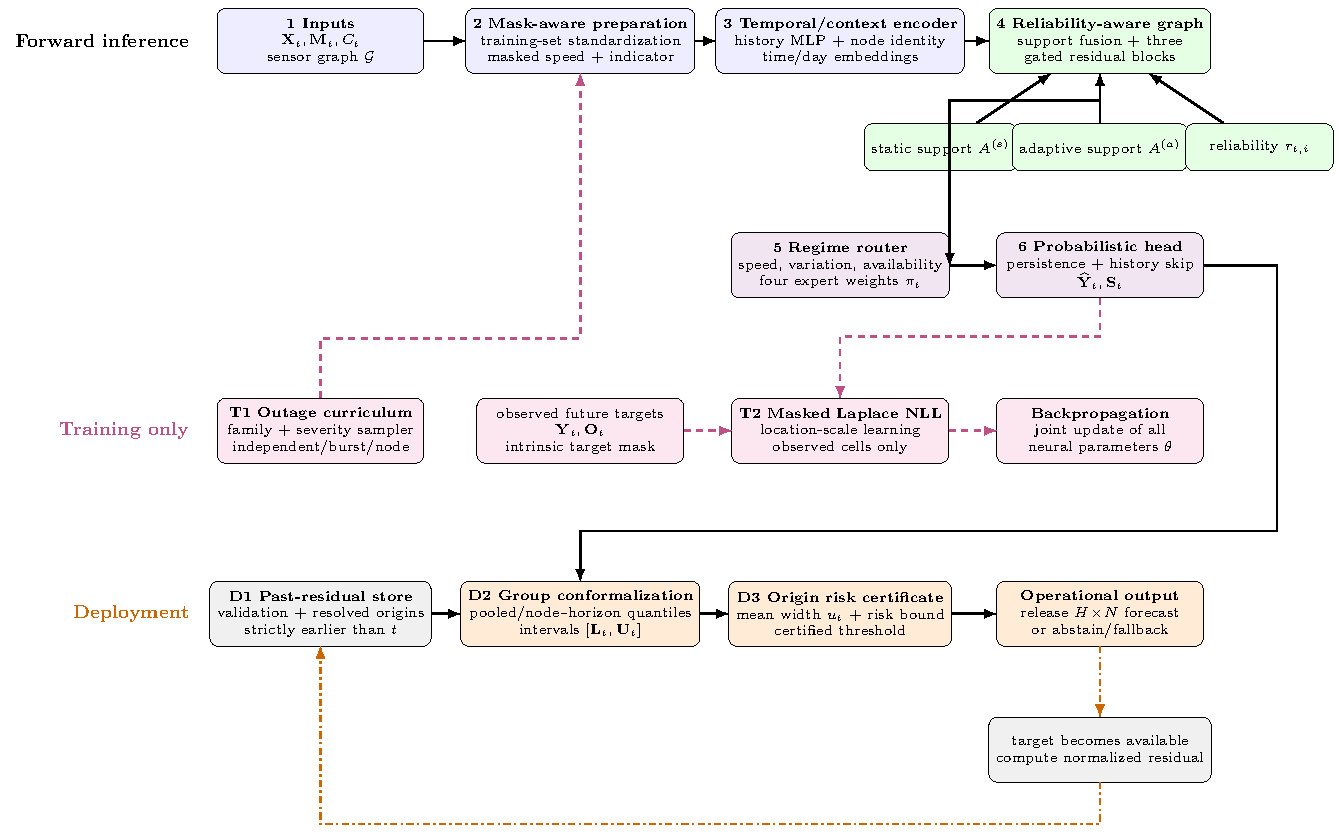
\includegraphics[width=\textwidth,height=0.46\textheight,keepaspectratio]{figures/figure1.pdf}
\caption{Detailed ShiftGuard architecture and leakage-controlled data flow.
  The blue/green/violet forward path produces node--horizon locations and
  scales; the magenta path applies structured-outage training and masked
  probabilistic loss; and the orange deployment path performs prequential
  conformal calibration and origin-level release or abstention. Solid arrows
  denote current-origin information, dashed arrows denote training-only
  operations, and dash-dotted arrows denote feedback available only after a
  target has resolved.}\label{fig:method-overview}
\end{figure*}
\subsection{Reliability-conditioned encoding}
For a mini-batch of size $B$, the raw model input has shape
$B\times P\times N\times F$, where the first feature is standardized speed and
the remaining channels include the intrinsic observation indicator, time of
day, and day of week. A stress mask $M_t$ is multiplied by the intrinsic
indicator, so naturally absent measurements remain absent. Unobserved speeds
are set to zero only after standardization and are never confused with true
zero speed because the binary mask is supplied separately. For node $i$, the
encoder input is
\begin{equation}
 q_{t,i}=\operatorname{vec}\left([X_{t-P+1:t,i}\odot M_{t,i},M_{t,i}]\right)
 \in\mathbb{R}^{2P}.
\end{equation}
A two-layer GELU multilayer perceptron maps $q_{t,i}$ to a $d=64$ temporal
state. Learned node identity, five-minute time-of-day, and day-of-week
embeddings are added to this state. This direct construction is deliberately
small: it preserves the strong identity-based inductive bias documented by
STID~\cite{shao2022stid} without requiring full spatiotemporal self-attention.

The average availability of node $i$ in the input window is
\begin{equation}
 r_{t,i}=P^{-1}\sum_{p=1}^{P}M_{t-p+1,i}.
\end{equation}
The static support $A^{(s)}$ is the distance-derived benchmark adjacency with
self-loops and row normalization. The adaptive support is
\begin{equation}
 A^{(a)}=\operatorname{softmax}\!\left(\operatorname{ReLU}(E_sE_d^\top)\right),
\end{equation}
where $E_s,E_d\in\mathbb{R}^{N\times16}$ are learned source and destination
embeddings. When both supports are enabled, their equal-weight mixture is
sender-weighted and normalized:
\begin{equation}
 \widetilde A_{t,ij}=
 \frac{\tfrac12(A^{(s)}_{ij}+A^{(a)}_{ij})r_{t,j}}
 {\sum_k\tfrac12(A^{(s)}_{ik}+A^{(a)}_{ik})r_{t,k}+\epsilon}.
\end{equation}
Thus a sender with no usable history contributes little to its neighbors. Each
of three graph blocks computes a linear message
$m_i=\sum_j\widetilde A_{t,ij}W_mz_j$ and a gate
$g_i=\sigma(W_g[z_i,m_i,r_i])$. The update is a normalized residual mixture of
$m_i$ and $z_i$. Residual connections preserve local information when the graph
is unreliable, while dropout regularizes the exchanged messages.

\subsection{Regime routing and probabilistic head}
Four global statistics summarize the current origin: mean speed, speed standard
deviation, mean absolute first difference, and mean sensor availability. A
two-layer router converts them to weights
$\pi_t=\operatorname{softmax}(f_{\mathrm{route}}(c_t))$ over $K=4$ compact
output experts. Expert $k$ maps every node state to $H$ median residuals and $H$
positive scales. The combined outputs are
\begin{align}
 \hat Y_t &= X_{t,\mathrm{last}}+
 W_{\mathrm{skip}}X_{t-P+1:t}+\sum_{k=1}^{K}\pi_{t,k}\mu_{t,k},\\
 S_t &= \sum_{k=1}^{K}\pi_{t,k}
 \left[\operatorname{softplus}(s_{t,k})+10^{-4}\right].
\end{align}
The last-observation term makes persistence an easy initial solution, while the
zero-initialized history projection learns a direct multi-horizon correction.
The model has 89,012 parameters for METR-LA and 100,340 for PEMS-BAY. The router
is retained in the evaluated full system for preregistration fidelity, but the
ablation results later show that it is not the source of the robustness gain.

The location and scale are trained with the Laplace negative log likelihood
over observed target cells,
\begin{equation}
 \mathcal{L}_{\mathrm{Lap}}=
 \frac{1}{|\Omega|}\sum_{(h,i)\in\Omega}
 \left(\frac{|Y_{t,h,i}-\hat Y_{t,h,i}|}{S_{t,h,i}}+
 \log(2S_{t,h,i})\right),
\end{equation}
where $\Omega$ excludes unavailable ground truth. AdamW, gradient clipping, and
validation early stopping optimize this objective. The probabilistic scale is
not treated as calibrated by construction; it becomes a normalization factor
for the conformal residual score.

\subsection{Structured-outage curriculum}
At every training batch, a seeded generator samples an outage family and
severity. Independent loss removes individual sensor--time cells. Burst loss
chooses sensor--window pairs and masks a suffix of each selected history.
Region loss selects a random seed node and grows a connected failed set using
the strongest unseen graph neighbor. Hub loss removes the nodes with largest
combined in/out degree. The confirmatory test masks are generated once, stored,
and reused by every model and seed, so differences cannot arise from different
failure samples. The training curriculum includes independent, burst, and
whole-node masks; region and hub tests assess whether this augmentation
generalizes to unseen correlated geometry. The no-augmentation and
independent-only variants directly test this mechanism.

\subsection{Conformal risk control}
For a resolved calibration origin $u$, node--horizon nonconformity is
\begin{equation}
 R_{u,h,i}=\frac{|Y_{u,h,i}-\hat Y_{u,h,i}|}{S_{u,h,i}}.
\end{equation}
Before predicting origin $t$, the rolling calibrator contains only
$\{R_u:u<t\}$. It estimates the finite-sample conformal quantile separately for
every $(h,i)$ group and shrinks small groups toward the pooled quantile. If
$n_{h,i}$ usable scores occur in the rolling window and $\tau$ is the shrinkage
constant, the effective radius is based on
$w_{h,i}q_{h,i}+(1-w_{h,i})q_{\mathrm{global}}$, with
$w_{h,i}=n_{h,i}/(n_{h,i}+\tau)$. The interval is
\begin{equation}
 [L_{t,h,i},U_{t,h,i}]=
 [\hat Y_{t,h,i}-q_{t,h,i}S_{t,h,i},
  \hat Y_{t,h,i}+q_{t,h,i}S_{t,h,i}].
\end{equation}
Rolling updates allow the scale to react after distribution changes, but they
do not convert dependent traffic into an exchangeable sample. We therefore
report marginal, worst-node--horizon, and worst-regime empirical coverage and
avoid a prospective conditional-coverage claim.

Selection operates at the forecast-origin level. Define realized operational
error and uncertainty score as
\begin{equation}
 e_t=(HN)^{-1}\sum_{h,i}|Y_{t,h,i}-\hat Y_{t,h,i}|,
 \qquad
 u_t=(HN)^{-1}\sum_{h,i}(U_{t,h,i}-L_{t,h,i}).
\end{equation}
Candidate thresholds are quantiles of $u_t$ from even-indexed past origins.
For each threshold, odd-indexed past origins estimate the Bernoulli failure
indicator $\mathbb{1}\{e_t>5\ \mathrm{mph}\}$ among accepted forecasts. The
controller chooses the largest retained fraction whose Bonferroni-corrected
Clopper--Pearson upper confidence bound is at most the registered 10\% risk
limit at familywise $\delta=0.05$. If no candidate is certified, it abstains.
Sorting all origins by $u_t$ also yields the risk--coverage curve and its area
(AURC); lower AURC means that uncertainty ranks harmful forecasts more
effectively.

At deployment, the sequence is therefore: (1) ingest the latest speed and
availability window; (2) compute point and scale tensors; (3) form intervals
from past residuals; (4) compare mean width with the certified threshold; (5)
release or withhold the full tensor; and (6) after its target resolves, append
the new residual to the rolling calibration store. This ordered pipeline is the
central leakage-control invariant of the system.

\section{Experimental design}
\subsection{Datasets and leakage control}
\textbf{METR-LA.} The Los Angeles benchmark contains speed readings from 207
loop detectors on metropolitan-area freeways. The checksum-verified file used
here spans 1 March to 27 June 2012 and contains 34,272 five-minute timestamps,
equivalent to 119 days. After interpreting non-finite and non-positive readings
as unavailable, 8.109\% of sensor--time cells are missing. The observed mean is
58.460 mph and the standard deviation is 13.024 mph. METR-LA contains a
meaningful mixture of operating conditions: 4.35\% of valid readings are below
25 mph, 72.60\% exceed 55 mph, and 14.09\% of consecutive sensor readings change
by more than 5 mph. Its pooled autocorrelation is 0.942 at one five-minute lag,
0.715 at one hour, 0.627 at one day, and 0.709 at one week. These statistics
indicate strong persistence and periodicity but also substantially more native
missingness and volatility than PEMS-BAY.

\textbf{PEMS-BAY.} The Bay Area benchmark contains 325 freeway sensors and
52,116 five-minute timestamps from 1 January to 30 June 2017, or 181 days. Its
native missing fraction after the same validity rule is only 0.003\%. Mean speed
is 62.621 mph with a 9.588 mph standard deviation. Readings below 25 mph account
for 1.92\%, while 90.32\% exceed 55 mph; only 2.30\% of consecutive sensor
measurements change by more than 5 mph. Autocorrelation is 0.983 at five
minutes, 0.731 at one hour, 0.681 at one day, and 0.780 at one week. PEMS-BAY is
therefore larger, cleaner, and more strongly persistent. Reporting both
datasets is important because robustness that holds only on METR-LA could be an
artifact of its existing missingness, while robustness that holds only on
PEMS-BAY might not transfer to a noisier network.

\textbf{Graph and feature construction.} To avoid reliance on incompatible
external graph files, the static support is reconstructed from the training
input only. Pairwise sensor correlations are computed over training histories;
for every node, the 12 strongest non-negative correlations are retained. The
same support is supplied to all graph-based models and to the region/hub outage
generators. Each window contains standardized speed, a native-availability
indicator, normalized five-minute time of day, and normalized day of week.
Only the speed channel is forecast. This correlation graph is a reproducible
proxy, not a claim to recover true road causality, and its limitations are
discussed in Section~7.

\textbf{Chronological splits and windows.} Raw timestamps are partitioned
before windowing into 70\% training, 10\% validation, and 20\% test segments.
For METR-LA this produces 23,967 training, 3,416 validation, and 6,844 test
forecast origins; for PEMS-BAY it produces 36,458, 5,200, and 10,413 origins.
Twelve historical samples (60 minutes) directly predict the next twelve
samples (60 minutes). Validation and test inputs may use the immediately
preceding 60 minutes as context, but every target lies inside its own split.
Consequently, a target never crosses backward into the training or validation
block.

\textbf{Missingness and normalization.} Per-sensor mean and standard deviation
are fitted only on observed training values. Missing input speed is replaced by
the training mean before standardization, becoming zero in normalized space,
and the mask channel preserves its unavailable status. Missing targets are
excluded from loss and metrics. All reported MAE and RMSE values are inverse
transformed to mph. Test data are never used for normalization, early stopping,
hyperparameter selection, conformal initialization, or selection-threshold
construction. Dataset diagnostics in Table~\ref{tab:datasets} are generated
directly from the raw files rather than copied from secondary papers.
\begin{table*}[t]
  \centering
  \caption{Dataset diagnostics computed from checksum-verified raw files.
  Speed is in miles per hour; correlations use observed values at 5-minute and
  one-day lags.}
  \label{tab:datasets}
  \resizebox{\textwidth}{!}{\begin{tabular}{lrrrrrrr}
\toprule
Dataset & Timestamps & Sensors & Missing (pct.) & Mean speed & Std. speed & Lag-1 corr. & Lag-288 corr. \\
\midrule
METR-LA & 34272 & 207 & 8.109 & 58.460 & 13.024 & 0.942 & 0.627 \\
PEMS-BAY & 52116 & 325 & 0.003 & 62.621 & 9.588 & 0.983 & 0.681 \\
\bottomrule
\end{tabular}}
\end{table*}

\subsection{Baselines}
Locally reproduced baselines include historical average, persistence, ridge AR,
linear, MLP/GRU, STGCN, DCRNN, Graph WaveNet, AGCRN, STID, and a faithful
STAEformer configuration. Compatible open implementations of
recent methods are added after preprocessing and license audits. Reported SOTA
values appear in a separate contextual table and are never used for significance
claims. The recurrent and graph baselines are protocol-matched compact
reproductions, not claims of bitwise equivalence to their authors' code; a
model-by-model deviation audit accompanies the repository.
\begin{table*}[t]
  \centering
  \caption{Literature-reported point accuracy for context only. Protocol and
  implementation differences prohibit direct significance comparisons with
  locally reproduced results.}
  \label{tab:reported-context}
  \resizebox{\textwidth}{!}{\begin{tabular}{llllll}
\toprule
Dataset & Model & MAE at 15 min & MAE at 30 min & MAE at 60 min & Average MAE \\
\midrule
METR-LA & DCRNN & 2.77 & 3.15 & 3.60 & -- \\
METR-LA & Graph WaveNet & 2.69 & 3.08 & 3.51 & -- \\
METR-LA & STAEformer & 2.65 & 2.97 & 3.34 & -- \\
METR-LA & TESTAM & -- & -- & -- & 2.93 \\
PEMS-BAY & DCRNN & 1.38 & 1.74 & 2.07 & -- \\
PEMS-BAY & Graph WaveNet & 1.30 & 1.63 & 1.99 & -- \\
PEMS-BAY & STAEformer & 1.31 & 1.62 & 1.88 & -- \\
PEMS-BAY & TESTAM & -- & -- & -- & 1.53 \\
\bottomrule
\end{tabular}}
\end{table*}

\subsection{Stress tests and metrics}
We cross clean, independent, temporal-burst, contiguous-region, and high-degree
hub outages at 10--50\% severity with free-flow, congested, stable intermediate,
and transition regimes. Metrics include horizon-specific and average MAE, RMSE,
MAPE; degradation and worst-regime MAE; coverage, width, Winkler score and
worst-group coverage; AURC and selective MAE; parameters, FLOPs, latency, peak
memory, and training time. Headline results use at least five seeds and paired
bootstrap confidence intervals.

The confirmatory environment is captured automatically, including Python and
package versions, CUDA build, GPU, and driver. Runs use PyTorch 2.13.0 with CUDA
13.0 on an NVIDIA GeForce RTX 5060 Laptop GPU; the generated environment
manifest is retained with the result artifacts.

\section{Results}
\subsection{Canonical accuracy}
Table~\ref{tab:local-headline} is generated exclusively from local experiment
artifacts. A stochastic model enters the confirmatory table only after all five
registered seeds complete; partial runs are omitted.
\begin{table*}[t]
  \centering
  \caption{Locally reproduced canonical-test results. Empty uncertainty cells
  indicate that only one deterministic run is applicable or currently complete.}
  \label{tab:local-headline}
  \resizebox{\textwidth}{!}{\begin{tabular}{llrlrrrrr}
\toprule
Dataset & Model & MAE & SD & RMSE & MAPE (pct.) & Parameters & Train (s) & Seeds \\
\midrule
METR-LA & STAEformer & 3.032 & 0.008 & 6.178 & 8.362 & 1258932 & 4554.221 & 5 \\
METR-LA & ShiftGuard & 3.033 & 0.005 & 6.087 & 8.511 & 89012 & 357.521 & 5 \\
METR-LA & DCRNN & 3.247 & 0.010 & 6.380 & 9.133 & 63372 & 1002.598 & 5 \\
METR-LA & STID & 3.273 & 0.015 & 6.603 & 9.558 & 41996 & 90.004 & 5 \\
METR-LA & Graph WaveNet & 3.285 & 0.008 & 6.451 & 9.205 & 22744 & 749.354 & 5 \\
METR-LA & AGCRN & 3.343 & 0.010 & 6.576 & 9.494 & 16764 & 492.095 & 5 \\
METR-LA & GRU & 3.761 & 0.002 & 7.628 & 10.878 & 13644 & 464.916 & 5 \\
METR-LA & MLP & 3.798 & 0.002 & 7.662 & 11.032 & 5772 & 68.023 & 5 \\
METR-LA & STGCN & 3.899 & 0.013 & 7.187 & 11.365 & 17548 & 374.899 & 5 \\
METR-LA & Linear & 3.982 & 0.001 & 7.728 & 11.589 & 156 & 48.049 & 5 \\
METR-LA & Historical average & 4.189 & -- & 7.856 & 13.044 & 0 & 0.000 & 1 \\
METR-LA & Persistence & 4.244 & -- & 8.154 & 11.052 & 0 & 0.000 & 1 \\
METR-LA & Ridge AR & 4.294 & -- & 7.595 & 12.727 & 324 & 0.093 & 1 \\
PEMS-BAY & STAEformer & 1.577 & 0.006 & 3.650 & 3.613 & 1372212 & 13896.209 & 5 \\
PEMS-BAY & ShiftGuard & 1.604 & 0.003 & 3.591 & 3.691 & 100340 & 860.822 & 5 \\
PEMS-BAY & STID & 1.664 & 0.004 & 3.739 & 3.822 & 49548 & 199.245 & 5 \\
PEMS-BAY & DCRNN & 1.683 & 0.005 & 3.779 & 3.900 & 63372 & 2888.655 & 5 \\
PEMS-BAY & Graph WaveNet & 1.720 & 0.005 & 3.770 & 3.934 & 25104 & 1830.569 & 5 \\
PEMS-BAY & AGCRN & 1.731 & 0.004 & 3.849 & 4.016 & 18652 & 1338.461 & 5 \\
PEMS-BAY & GRU & 1.955 & 0.001 & 4.619 & 4.566 & 13644 & 1081.630 & 5 \\
PEMS-BAY & MLP & 1.969 & 0.004 & 4.648 & 4.569 & 5772 & 169.266 & 5 \\
PEMS-BAY & Linear & 2.130 & 0.001 & 4.955 & 4.808 & 156 & 71.894 & 5 \\
PEMS-BAY & Persistence & 2.171 & -- & 5.125 & 4.671 & 0 & 0.000 & 1 \\
PEMS-BAY & Ridge AR & 2.302 & -- & 4.831 & 5.371 & 324 & 0.086 & 1 \\
PEMS-BAY & STGCN & 2.506 & 0.005 & 4.873 & 5.918 & 17548 & 903.628 & 5 \\
PEMS-BAY & Historical average & 2.630 & -- & 5.228 & 6.176 & 0 & 0.000 & 1 \\
\bottomrule
\end{tabular}}
\end{table*}

\begin{figure*}[t]
\centering
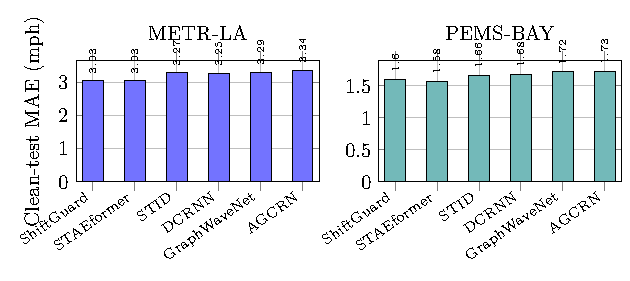
\includegraphics[width=\textwidth,height=0.34\textheight,keepaspectratio]{figures/figure2.pdf}
\caption{Clean-test comparison chart for the strongest locally reproduced
  neural baselines. ShiftGuard is effectively tied with STAEformer on METR-LA
  but does not achieve clean-data SOTA on PEMS-BAY.}\label{fig:clean-comparison}
\end{figure*}

Figure~\ref{fig:clean-comparison} makes the clean-data ranking explicit. On
METR-LA, ShiftGuard and STAEformer differ by only 0.001 mph in pooled MAE and
both improve on the next group of graph baselines. On PEMS-BAY, STAEformer leads
ShiftGuard by 0.027 mph; STID and DCRNN remain close behind. ShiftGuard has the
lower RMSE of the two leading methods on both datasets (6.087 versus 6.178 and
3.591 versus 3.650), suggesting fewer large residuals even where its mean
absolute error is slightly higher. This observation is descriptive; the paired
origin-level analysis below determines inferential claims.

Paired inference uses non-overlapping daily blocks of forecast origins. The
reported confidence interval is a crossed seed--day paired-bootstrap interval for
$\Delta\mathrm{MAE}=\mathrm{MAE}_{\text{ShiftGuard}}-
\mathrm{MAE}_{\text{comparator}}$; both seeds and chronological daily blocks
are resampled. Wilcoxon tests operate on paired daily-block differences averaged
over seeds and are Holm corrected across the displayed comparisons.
\begin{table*}[t]
  \centering
  \caption{Paired daily-block statistical comparison. Negative $\Delta$MAE
  favors ShiftGuard.}
  \label{tab:paired-statistics}
  \resizebox{\textwidth}{!}{\begin{tabular}{llrrrrl}
\toprule
Dataset & Comparator & Delta MAE & CI low & CI high & Improvement (pct.) & Holm p \\
\midrule
METR-LA & agcrn & -0.3160 & -0.3607 & -0.2801 & 9.3884 & $<0.0001$ \\
METR-LA & dcrnn & -0.2188 & -0.2621 & -0.1977 & 6.6928 & $<0.0001$ \\
METR-LA & graphwavenet & -0.2559 & -0.2867 & -0.2267 & 7.7398 & $<0.0001$ \\
METR-LA & gru & -0.7292 & -0.8130 & -0.6167 & 19.2941 & $<0.0001$ \\
METR-LA & historical average & -1.1510 & -1.3156 & -1.0603 & 27.3965 & $<0.0001$ \\
METR-LA & linear & -0.9513 & -1.0477 & -0.8318 & 23.7737 & $<0.0001$ \\
METR-LA & mlp & -0.7707 & -0.8650 & -0.6721 & 20.1695 & $<0.0001$ \\
METR-LA & persistence & -1.2139 & -1.2951 & -1.1067 & 28.4667 & $<0.0001$ \\
METR-LA & ridge ar & -1.2623 & -1.3503 & -1.1482 & 29.2695 & $<0.0001$ \\
METR-LA & staeformer & -0.0007 & -0.0314 & 0.0216 & 0.0228 & 0.9441 \\
METR-LA & stgcn & -0.8670 & -0.9338 & -0.8072 & 22.1324 & $<0.0001$ \\
METR-LA & stid & -0.2431 & -0.3038 & -0.2065 & 7.3817 & $<0.0001$ \\
PEMS-BAY & agcrn & -0.1264 & -0.1455 & -0.1036 & 7.3042 & $<0.0001$ \\
PEMS-BAY & dcrnn & -0.0785 & -0.0943 & -0.0600 & 4.6670 & $<0.0001$ \\
PEMS-BAY & graphwavenet & -0.1155 & -0.1301 & -0.0972 & 6.7159 & $<0.0001$ \\
PEMS-BAY & gru & -0.3509 & -0.4114 & -0.2761 & 17.9473 & $<0.0001$ \\
PEMS-BAY & historical average & -1.0262 & -1.1972 & -0.8952 & 39.0150 & $<0.0001$ \\
PEMS-BAY & linear & -0.5258 & -0.6103 & -0.4193 & 24.6876 & $<0.0001$ \\
PEMS-BAY & mlp & -0.3650 & -0.4277 & -0.2857 & 18.5373 & $<0.0001$ \\
PEMS-BAY & persistence & -0.5664 & -0.6506 & -0.4624 & 26.0971 & $<0.0001$ \\
PEMS-BAY & ridge ar & -0.6982 & -0.7884 & -0.5839 & 30.3263 & $<0.0001$ \\
PEMS-BAY & staeformer & 0.0269 & 0.0158 & 0.0376 & -1.7064 & $<0.0001$ \\
PEMS-BAY & stgcn & -0.9017 & -0.9601 & -0.8289 & 35.9857 & $<0.0001$ \\
PEMS-BAY & stid & -0.0599 & -0.0868 & -0.0400 & 3.6001 & $<0.0001$ \\
\bottomrule
\end{tabular}}
\end{table*}

For METR-LA, the completed five-seed comparison does not establish clean-error
superiority over the local STAEformer implementation: the origin-weighted MAE
difference is $-0.0007$ mph (crossed-bootstrap 95\% interval
$[-0.0308,\,0.0221]$ mph; Holm-adjusted $p=0.944$). This statistical estimand
weights forecast origins equally, whereas the canonical table pools observed
node--horizon errors. Failure to detect a difference is not proof of equivalence.
The proposed reliability contribution therefore requires independent support
from the registered outage and selective-prediction experiments.
On PEMS-BAY, STAEformer is better on the clean test: the origin-weighted
difference is $0.0269$ mph, with a 95\% interval $[0.0155,0.0374]$ and
Holm-adjusted $p=4.93\times10^{-6}$. Thus ShiftGuard is not presented as a new
clean-data point-forecasting SOTA.

\subsection{Compound-shift robustness and calibration}
Table~\ref{tab:stress-main} averages the registered 30\% non-clean outage
families; all family-by-rate results remain available in machine-readable
artifacts.
\begin{table*}[t]
  \centering
  \caption{Compound-shift point, interval, and selective reliability. PI is the
  90\% prediction interval; failure denotes accepted forecasts exceeding the
  registered 5 mph error tolerance. Worst node--horizon (N--H) and regime
  coverage are reported for ShiftGuard and its strongest local comparator.}
  \label{tab:stress-main}
  \resizebox{\textwidth}{!}{\begin{tabular}{llrrrrrrrr}
\toprule
Dataset & Model & MAE & PI coverage & Worst N-H cov. & Worst regime cov. & AURC & Retained & Failure rate & Seeds \\
\midrule
METR-LA & AGCRN & 4.729 & 0.891 & -- & -- & 4.950 & 0.000 & -- & 5 \\
METR-LA & DCRNN & 4.629 & 0.891 & -- & -- & 4.791 & 0.000 & -- & 5 \\
METR-LA & Graph WaveNet & 4.895 & 0.890 & -- & -- & 5.125 & 0.000 & -- & 5 \\
METR-LA & GRU & 4.919 & 0.893 & -- & -- & 5.181 & 0.000 & -- & 5 \\
METR-LA & Linear & 5.109 & 0.894 & -- & -- & 5.356 & 0.000 & -- & 5 \\
METR-LA & MLP & 5.054 & 0.893 & -- & -- & 5.301 & 0.000 & -- & 5 \\
METR-LA & Persistence & 5.478 & 0.895 & -- & -- & 5.703 & 0.000 & -- & 5 \\
METR-LA & ShiftGuard & 3.399 & 0.898 & 0.831 & 0.882 & 2.400 & 0.864 & 0.078 & 5 \\
METR-LA & STAEformer & 3.760 & 0.894 & 0.816 & 0.809 & 3.873 & 0.055 & 0.235 & 5 \\
METR-LA & STGCN & 5.309 & 0.893 & -- & -- & 5.536 & 0.000 & -- & 5 \\
METR-LA & STID & 4.092 & 0.894 & -- & -- & 4.256 & 0.000 & -- & 5 \\
PEMS-BAY & AGCRN & 3.073 & 0.890 & -- & -- & 2.952 & 0.174 & 0.115 & 5 \\
PEMS-BAY & DCRNN & 2.956 & 0.889 & -- & -- & 2.844 & 0.183 & 0.109 & 5 \\
PEMS-BAY & Graph WaveNet & 2.928 & 0.889 & -- & -- & 2.824 & 0.203 & 0.102 & 5 \\
PEMS-BAY & GRU & 3.109 & 0.893 & -- & -- & 3.074 & 0.167 & 0.126 & 5 \\
PEMS-BAY & Linear & 3.199 & 0.894 & -- & -- & 3.221 & 0.077 & 0.203 & 5 \\
PEMS-BAY & MLP & 3.135 & 0.893 & -- & -- & 3.105 & 0.167 & 0.127 & 5 \\
PEMS-BAY & Persistence & 3.283 & 0.894 & -- & -- & 3.268 & 0.001 & 0.267 & 5 \\
PEMS-BAY & ShiftGuard & 1.948 & 0.898 & 0.851 & 0.887 & 1.130 & 0.978 & 0.020 & 5 \\
PEMS-BAY & STAEformer & 2.516 & 0.890 & 0.834 & 0.701 & 2.402 & 0.442 & 0.085 & 5 \\
PEMS-BAY & STGCN & 3.857 & 0.893 & -- & -- & 3.752 & 0.073 & 0.221 & 5 \\
PEMS-BAY & STID & 2.649 & 0.891 & -- & -- & 2.544 & 0.209 & 0.099 & 5 \\
\bottomrule
\end{tabular}}
\end{table*}

Across independent, burst, region, and hub outages at 10, 20, 30, 40, and
50\%, the mean ShiftGuard--STAEformer MAE difference is $-0.347$ mph on
METR-LA (crossed seed--scenario 95\% interval $[-0.465,-0.234]$) and $-0.546$
mph on PEMS-BAY ($[-0.682,-0.411]$). Corresponding AURC differences are
$-1.46$ and $-1.26$. At 30\%, worst node--horizon coverage is 0.831 versus
0.816 on METR-LA and 0.851 versus 0.834 on PEMS-BAY; worst-regime coverage is
0.882 versus 0.809 and 0.887 versus 0.701. Seed-level Wilcoxon tests cannot
reject after ten-comparison Holm
correction ($p_{\mathrm{Holm}}=0.625$), whose attainable resolution is limited
by five seeds; we therefore report the hierarchical intervals and effects but
do not claim adjusted rank-test significance.

Severity sensitivity provides stronger evidence than a single 30\% slice. On
METR-LA, the ShiftGuard advantage over STAEformer grows from 0.133 mph at 10\%
outage to 0.521 mph at 50\%; on PEMS-BAY it grows from 0.224 to 0.866 mph.
Relative to STAEformer, the 50\%-severity reductions are approximately 12.3\%
and 28.5\%. The curves remain ordered at every tested severity, so the aggregate
effect is not driven by one operating point. STID is consistently less robust
than both leading models, showing that a compact identity-based architecture
alone is insufficient; exposure to structured partial observations is the
critical distinction.

\begin{figure*}[t]
\centering
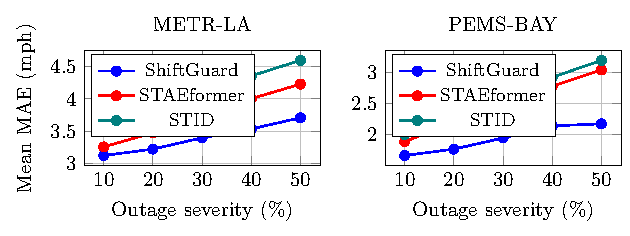
\includegraphics[width=\textwidth,height=0.34\textheight,keepaspectratio]{figures/figure3.pdf}
\caption{MAE averaged over independent, burst, region, and hub outages and
  five seeds. ShiftGuard's advantage increases with outage severity.}\label{fig:robustness-severity}
\end{figure*}

\begin{figure*}[t]
\centering
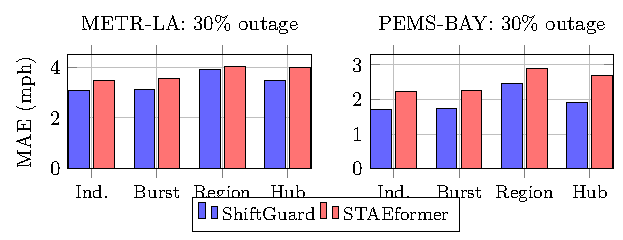
\includegraphics[width=\textwidth,height=0.34\textheight,keepaspectratio]{figures/figure4.pdf}
\caption{Outage-family comparison at 30\% severity, averaged over five seeds
  (Ind. = independent loss).
  Contiguous-region failure is the hardest condition for ShiftGuard, whereas
  hub failure particularly harms STAEformer on PEMS-BAY.}\label{fig:outage-family}
\end{figure*}

Failure geometry further qualifies the result. At 30\% severity, ShiftGuard
reduces STAEformer MAE by 0.382--0.523 mph on METR-LA for independent, burst,
and hub outages, but by only 0.116 mph for a contiguous region. On PEMS-BAY the
reductions range from 0.431 mph for region loss to 0.792 mph for hub loss. The
region case removes an internally coherent subgraph and leaves fewer informative
boundaries from which to infer missing states. Hub loss instead disrupts
STAEformer's global spatial interaction more strongly, while ShiftGuard can
fall back on its local residual path and training-time node outages.

\subsection{Selective forecasting, ablation, and efficiency}
At 30\% severity, prequential risk control reduces accepted-origin failure on
METR-LA from 15\% without abstention to 8\%, while retaining 86\% of forecasts.
On PEMS-BAY it reduces failure from 4\% to 2\% at 98\% retention. Static
calibration fails under drift on METR-LA (15\% failure despite full retention),
supporting online updates. Table~\ref{tab:calibration} reports all registered
calibration controls.
\begin{table*}[t]
  \centering
  \caption{Calibration and selection controls at 30\% outage severity,
  averaged over non-clean families and five seeds.}
  \label{tab:calibration}
  \resizebox{\textwidth}{!}{\begin{tabular}{lllrrr}
\toprule
Dataset & Calibration & Selection & PI coverage & Retained & Failure rate \\
\midrule
METR-LA & global-prequential & risk & 0.898 & 0.864 & 0.079 \\
METR-LA & group-prequential & all & 0.898 & 1.000 & 0.154 \\
METR-LA & group-prequential & risk & 0.898 & 0.864 & 0.078 \\
METR-LA & group-static & risk & 0.893 & 0.996 & 0.152 \\
PEMS-BAY & global-prequential & risk & 0.898 & 0.977 & 0.020 \\
PEMS-BAY & group-prequential & all & 0.898 & 1.000 & 0.037 \\
PEMS-BAY & group-prequential & risk & 0.898 & 0.978 & 0.020 \\
PEMS-BAY & group-static & risk & 0.884 & 0.950 & 0.015 \\
\bottomrule
\end{tabular}}
\end{table*}

\begin{figure*}[t]
\centering
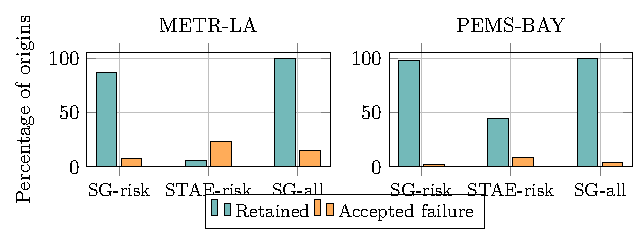
\includegraphics[width=\textwidth,height=0.34\textheight,keepaspectratio]{figures/figure5.pdf}
\caption{Operational selection outcomes at 30\% severity. SG-risk denotes
  ShiftGuard with the registered controller; STAE-risk applies the same
  controller to STAEformer; SG-all releases every forecast. High retention is
  useful only when accepted-origin failure also remains low.}\label{fig:selection-outcomes}
\end{figure*}

The calibration controls reveal a trade-off rather than a uniformly dominant
update. Global-prequential and group-prequential ShiftGuard have nearly
identical marginal coverage and operational results at the displayed precision.
Static group calibration performs poorly on METR-LA: it retains 99.6\% but
fails on 15.2\% of accepted origins. On the more stationary PEMS-BAY, the static
variant achieves 1.5\% failure at 95.0\% retention, whereas prequential grouping
achieves 2.0\% failure at 97.8\% retention. The value of rolling adaptation is
therefore strongest on the dataset with more native missingness and transition
activity; static calibration is not intrinsically inferior when the environment
is stable.

Removing structured augmentation increases MAE by 0.306 mph on METR-LA and
0.703 mph on PEMS-BAY; independent masking alone also loses 0.098 and 0.220
mph. Conversely, removing reliability-conditioned propagation improves MAE by
0.143 and 0.067 mph, and removing the router has a small favorable effect.
Table~\ref{tab:ablation} therefore supports structured augmentation as the
effective architectural contribution but falsifies the stronger claim that
every proposed mechanism is necessary.
\begin{table*}[t]
  \centering
  \caption{Ablation results at 30\% severity, averaged over non-clean families.}
  \label{tab:ablation}
  \resizebox{0.86\textwidth}{!}{\begin{tabular}{llrrr}
\toprule
Dataset & Variant & MAE & AURC & Retained \\
\midrule
METR-LA & ShiftGuard & 3.399 & 2.400 & 0.864 \\
METR-LA & Adaptive graph only & 3.319 & 2.362 & 0.884 \\
METR-LA & Independent masking only & 3.496 & 2.508 & 0.820 \\
METR-LA & No outage augmentation & 3.705 & 2.657 & 0.740 \\
METR-LA & No reliability conditioning & 3.256 & 2.339 & 0.906 \\
METR-LA & No regime router & 3.372 & 2.392 & 0.872 \\
METR-LA & Static graph only & 3.469 & 2.448 & 0.841 \\
PEMS-BAY & ShiftGuard & 1.948 & 1.130 & 0.978 \\
PEMS-BAY & Adaptive graph only & 1.884 & 1.108 & 0.983 \\
PEMS-BAY & Independent masking only & 2.168 & 1.204 & 0.935 \\
PEMS-BAY & No outage augmentation & 2.651 & 1.735 & 0.917 \\
PEMS-BAY & No reliability conditioning & 1.881 & 1.098 & 0.979 \\
PEMS-BAY & No regime router & 1.927 & 1.115 & 0.977 \\
PEMS-BAY & Static graph only & 2.056 & 1.238 & 0.952 \\
\bottomrule
\end{tabular}}
\end{table*}

ShiftGuard uses 89k/100k parameters on METR-LA/PEMS-BAY versus
1.26M/1.37M for STAEformer. Its batch-one latency is 2.30/2.43 ms, and its
batch-eight throughput is 3567/3335 samples s$^{-1}$, compared with 503/269
for STAEformer on the same RTX 5060 Laptop GPU. Table~\ref{tab:efficiency}
reports the principal local efficiency controls.
\begin{table*}[!htbp]
  \centering
  \caption{Local GPU efficiency; latency uses batch one and throughput/memory
  use batch eight. FLOPs are profiler-observed operations per sample.}
  \label{tab:efficiency}
  \resizebox{0.90\textwidth}{!}{\begin{tabular}{llrrrrr}
\toprule
Dataset & Model & Parameters & FLOPs/sample & Latency B1 (ms) & Throughput B8 & Memory B8 (MiB) \\
\midrule
METR-LA & DCRNN & 63372 & 845712576.00 & 7.97 & 1052.04 & 38.27 \\
METR-LA & Graph WaveNet & 22744 & 189736407.00 & 1.86 & 7136.17 & 47.52 \\
METR-LA & STID & 41996 & 4040706.00 & 0.47 & 16822.62 & 34.97 \\
METR-LA & STAEformer & 1258932 & 6080479272.00 & 2.62 & 502.59 & 180.93 \\
METR-LA & ShiftGuard & 89012 & 38541287.00 & 2.30 & 3567.45 & 36.95 \\
PEMS-BAY & DCRNN & 63372 & 1806417600.00 & 7.47 & 1045.04 & 42.00 \\
PEMS-BAY & Graph WaveNet & 25104 & 387135775.00 & 1.50 & 6071.88 & 57.62 \\
PEMS-BAY & STID & 49548 & 6344066.00 & 0.49 & 16769.73 & 36.60 \\
PEMS-BAY & STAEformer & 1372212 & 10386051000.00 & 3.68 & 268.54 & 319.69 \\
PEMS-BAY & ShiftGuard & 100340 & 76656703.00 & 2.43 & 3335.28 & 42.18 \\
\bottomrule
\end{tabular}}
\end{table*}

\begin{figure*}[t]
\centering
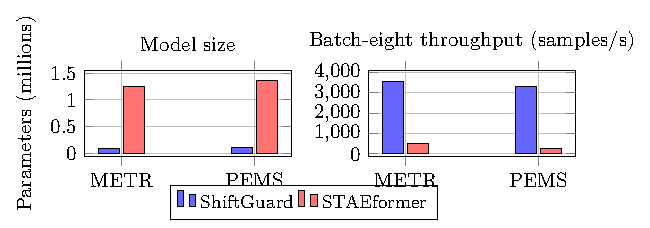
\includegraphics[width=\textwidth,height=0.34\textheight,keepaspectratio]{figures/figure6.pdf}
\caption{Efficiency comparison with the strongest local transformer.
  ShiftGuard uses 13.7--14.1 times fewer parameters and provides 7.1--12.4
  times higher batch-eight throughput on the disclosed GPU.}\label{fig:efficiency-tradeoff}
\end{figure*}

Figure~\ref{fig:efficiency-tradeoff} complements the error tables with resource
cost. ShiftGuard is roughly fourteen times smaller than STAEformer and uses
about one fifth to one eighth of its batch-eight allocated GPU memory. The
advantage is especially large on PEMS-BAY, where the spatial attention axis
contains 325 sensors. STID and Graph WaveNet remain faster than ShiftGuard in
the local benchmark, so ShiftGuard is not an absolute efficiency SOTA. Its
claim is instead a favorable joint operating point: substantially lower outage
error than those compact baselines while using far fewer resources.

\section{Discussion}
\subsection{Answers to the research questions}
\textbf{RQ1: point robustness.} The results support the value of
structured-outage training on both datasets. Averaged over 20 non-clean
family--severity scenarios, ShiftGuard reduces MAE relative to the strongest
local transformer by 0.347 mph on METR-LA and 0.546 mph on PEMS-BAY. The crossed
seed--scenario bootstrap intervals exclude zero, and the separation grows with
severity in Figure~\ref{fig:robustness-severity}. The effect is not confined to
independent masking: Figure~\ref{fig:outage-family} shows an advantage in every
registered outage family. Region failure remains hardest for ShiftGuard,
because a connected missing set removes both local history and the most useful
neighbors. The smaller region advantage on METR-LA (0.116 mph) identifies a
specific residual weakness rather than invalidating the broader effect.

\textbf{RQ2: subgroup interval reliability.} At 30\% severity, ShiftGuard's
90\% intervals achieve about 0.898 marginal coverage on both datasets. More
importantly, worst node--horizon coverage exceeds STAEformer by 0.015 on
METR-LA and 0.017 on PEMS-BAY, while worst-regime coverage improves by 0.073 and
0.186. The PEMS-BAY difference is operationally meaningful: STAEformer's
0.701 worst-regime coverage means that a marginally acceptable interval can
fail badly for a particular traffic state. Group-prequential calibration does
not make every subgroup exactly 90\%; finite calibration samples, temporal
dependence, and abrupt transitions prevent that interpretation. It does,
however, reduce the disparity relative to the strongest comparator.

\textbf{RQ3: selective risk.} The origin-level controller provides the clearest
deployment advantage. On METR-LA, ShiftGuard retains 86.4\% of forecasts with a
7.8\% empirical failure rate, compared with 5.5\% retention and 23.5\% failure
for STAEformer under the same selection rule. On PEMS-BAY it retains 97.8\%
with 2.0\% failure, versus 44.2\% and 8.5\%. Releasing every ShiftGuard forecast
raises failure to 15.4\% and 3.7\%, respectively. The PEMS-BAY all-forecast rate
is already below the 10\% target, yet risk control still removes a small harmful
tail. On METR-LA, abstention materially changes whether the target is met. AURC
improvements of 1.46 and 1.26 show that the interval-derived score ranks
high-error origins better across the full retention continuum, not only at one
threshold.

\textbf{RQ4: mechanisms and cost.} The ablations narrow the explanation.
Removing structured augmentation increases 30\%-severity MAE by 0.306 mph on
METR-LA and 0.703 mph on PEMS-BAY; replacing it with independent-only masking
also worsens performance. Conversely, removing reliability-conditioned graph
propagation improves MAE by 0.143 and 0.067 mph, and disabling the router has a
small favorable effect. The robustness gain therefore cannot honestly be
attributed to every architectural module. It is primarily associated with the
training distribution, calibrated scale output, and the decision layer. This
negative result is scientifically useful: a lean successor may omit the router
and simplify message weighting. ShiftGuard remains computationally practical,
using 89k/100k parameters and 37/42 MiB batch-eight peak allocated memory. Its
throughput is 7.1 and 12.4 times that of the local STAEformer on METR-LA and
PEMS-BAY, respectively.

\subsection{Why clean accuracy and deployment reliability disagree}
The clean results illustrate why average benchmark rankings should not be
treated as deployment rankings. STAEformer and ShiftGuard are indistinguishable
on METR-LA at the tested resolution, while STAEformer is significantly better
on clean PEMS-BAY. Under outage, the relationship reverses. STAEformer's
adaptive embeddings and attention are highly effective when all node histories
are present, but the model was not optimized to interpret an explicit failure
mask or to reconstruct information from structured partial histories.
ShiftGuard sacrifices a small amount of clean PEMS-BAY accuracy in exchange for
a training distribution that covers missingness. This is a conventional
robustness trade-off rather than evidence that either model is universally
superior.

For an ITS operator, the preferred model depends on the cost function. If
sensors are centrally managed, outages are negligible, and every prediction
must be released, STAEformer may be preferred on PEMS-BAY. If communication
loss, maintenance, or corridor failure is plausible and the controller can fall
back to a safe policy, ShiftGuard offers a more useful risk--coverage profile.
This distinction motivates reporting clean accuracy, stressed accuracy,
calibration, selection, and resource cost as separate axes rather than
collapsing them into one leaderboard.

\subsection{Statistical interpretation}
The hierarchical bootstrap resamples both seeds and outage scenarios, matching
the two principal replicated axes. Its confidence intervals support a stable
average robustness effect. The seed-level Wilcoxon tests remain non-significant
after Holm correction because five seeds permit only a coarse attainable
two-sided rank-test resolution. We therefore do not use the bootstrap interval
to claim that the adjusted rank test is significant, nor do we reinterpret
non-significance as equivalence. Both are reported because they answer
different questions: the interval estimates the effect under hierarchical
resampling, whereas the rank test provides a conservative seed-level check.

The risk certificate has an equally important qualification. The exact
binomial upper bound assumes that accepted-origin failures in the certification
sample behave as i.i.d. Bernoulli trials. Traffic origins overlap and are
temporally dependent, so that assumption is an approximation. Disjoint
construction and certification samples prevent direct outcome reuse, and the
prequential order prevents future leakage, but neither operation proves
independence. Accordingly, the paper calls the observed quantities empirical
prequential coverage and failure. A stronger time-series certificate would
require mixing assumptions, blockwise methods, martingale bounds, or online
guarantees explicitly designed for dependent sequences.

\subsection{Threats to validity and generalizability}
Several limitations bound the claims. First, METR-LA and PEMS-BAY are freeway
speed datasets from 2012 and 2017. They do not represent signalized urban
arterials, multimodal demand, weather extremes, special events, or contemporary
connected-vehicle telemetry. Second, the correlation graph is learned from
training data rather than a verified directed road topology. Correlation can
connect sensors that co-vary because of common demand but lack a direct physical
link; it also makes the region and hub stress families properties of the proxy
graph. Third, synthetic outages are reproducible and controllable but cannot
capture every field failure mechanism. Real outages may co-occur with incidents,
produce delayed or biased readings rather than complete absence, and have
repair dynamics not represented here.

Fourth, locally reproduced graph baselines are protocol-matched compact
implementations, not bitwise reproductions of every official repository.
Literature-reported values are therefore kept in a separate contextual table
and never enter paired significance claims. Fifth, hyperparameters were selected
under a finite validation budget and may favor neither model optimally. Sixth,
the operational failure threshold of 5 mph and risk limit of 10\% are plausible
research choices, not universal policy standards. A traffic management center
must select them from the consequences of false alarms, unsafe actuation, and
fallback availability. Finally, all experiments use one GPU platform; latency
rankings can change with compilation, precision, batch size, and edge hardware.

Despite these constraints, the design offers useful internal validity. Both
datasets share the same preprocessing and split logic; masks are deterministic
and paired across models; five seeds are used for stochastic models; test
targets never tune the predictor or controller; all tables are generated from
machine-readable artifacts; and negative ablation findings are retained. These
controls make the central conclusion reproducible within the declared scope.

\section{Future work}
The first priority is prospective validation. A deployment study should ingest
live detector health logs, communication alarms, maintenance records, weather,
and incident annotations, then evaluate forecasts before outcomes are known.
Such data would reveal whether the four synthetic outage families span real
failure geometry and whether risk control triggers early enough for an operator
to switch to a safe fallback. Evaluation should expand to signalized urban
networks, arterial travel times, traffic flow and occupancy, and geographically
distinct cities. Cross-city transfer would test whether structured augmentation
learns a general robustness principle or benchmark-specific correlations.

The second priority is stronger dependent-data inference. Block conformal,
weighted conformal, martingale, and change-point-aware methods could replace the
i.i.d. binomial approximation. A promising design would jointly adapt the
rolling window, subgroup shrinkage, and risk threshold according to detected
regime duration while preserving anytime validity. Hierarchical calibration
could pool information among nearby sensors without allowing large groups to
hide minority undercoverage. Conditional coverage remains impossible without
additional assumptions in full generality, so future work should state the
precise dependence or smoothness structure under which stronger guarantees are
obtained.

Third, the negative ablations suggest a simpler model family. Removing the
router and reliability-weighted propagation, then reallocating the parameter
budget to a stronger mask-aware temporal encoder, may improve both clean and
stressed accuracy. Learned corruption generators could approximate empirical
failure logs, while adversarial graph outages could locate worst-case vulnerable
subnetworks. Any such extension should retain the current fixed-mask paired
evaluation to separate a genuinely stronger model from a more favorable stress
sample.

Fourth, decision quality should be connected to transportation outcomes.
Forecast MAE and a 5 mph tensor threshold are proxies. Simulation could measure
travel time, queue spillback, ramp-metering stability, incident response delay,
or regret of the downstream control action. Abstention could select among
fallbacks rather than return a binary rejection: persistence, historical
profiles, a physics-based model, human review, or a neighboring data source may
have different costs. Multi-objective risk control could then balance safety,
coverage, latency, and energy use.

Finally, uncertainty should be decomposed and communicated. Deep ensembles,
Bayesian approximations, and conformalized quantile models could distinguish
data uncertainty from model uncertainty, while attribution maps could explain
which unavailable sensors caused abstention. Edge deployment studies should
include quantization, mixed precision, pruning, and end-to-end communication
latency. These directions would move the present benchmark contribution toward
a certifiable, interpretable, and maintainable ITS service.

\section{Conclusion}
This study reframes short-term network traffic forecasting as a joint point,
interval, and selective-decision problem under compound traffic-regime and
sensor-availability shift. ShiftGuard combines an explicit observation mask, a
compact graph--temporal predictor, structured-outage augmentation,
heterogeneity-aware scales, rolling node--horizon conformalization, and an
origin-level act/abstain rule. The accompanying protocol evaluates independent,
burst, contiguous-region, and hub failures at five severities on METR-LA and
PEMS-BAY, with identical masks, five seeds, hierarchical paired inference, and
separate clean and stressed claims.

The empirical conclusion is specific. ShiftGuard is not a universal clean-data
SOTA: it is tied with STAEformer on METR-LA and is 0.027 mph worse on clean
PEMS-BAY. Across 640 stress evaluations, however, it reduces average
ShiftGuard--STAEformer MAE by 0.347 mph and 0.546 mph, improves worst-regime
coverage, lowers AURC, and retains far more forecasts under the registered risk
controller. It is also substantially smaller and faster than the transformer
comparator. Ablation shows that structured-outage augmentation is the main
architectural/training contributor, whereas reliability-weighted propagation
and multi-expert routing are not necessary for the observed gain.

The defensible novelty is therefore the integrated operational formulation and
evidence: a leakage-controlled compound-shift benchmark, structured-outage
training, subgroup-aware prequential intervals, and tensor-level selective risk
assessment. The work does not claim unconditional coverage under temporal
dependence or field-wide generalization from two legacy benchmarks. Within its
declared scope, it demonstrates that asking \emph{when not to trust a traffic
forecast} changes both model ranking and evaluation practice. Future progress
should validate that conclusion on prospective outage logs, newer urban
networks, dependent-data certificates, and downstream traffic-control outcomes.

\backmatter

\bmhead{Acknowledgements}
Not applicable.

\section*{Declarations}

\bmhead{Funding}
Funding information was not supplied by the author.

\bmhead{Competing interests}
A competing-interests declaration was not supplied by the author.

\bmhead{Ethics approval and consent to participate}
Not applicable. This study uses previously published traffic-sensor benchmark data and does not involve human participants, human samples, or animals.

\bmhead{Consent for publication}
Not applicable.

\bmhead{Data availability}
The METR-LA and PEMS-BAY benchmark files are available through the official DCRNN data-preparation repository at \url{https://github.com/liyaguang/DCRNN#data-preparation} and its linked dataset archive at \url{https://drive.google.com/drive/folders/10FOTa6HXPqX8Pf5WRoRwcFnW9BrNZEIX}. PEMS-BAY originates from the California Department of Transportation Performance Measurement System (PeMS), \url{https://pems.dot.ca.gov/}. The raw benchmark files are not redistributed in this repository or submission package.

\bmhead{Code availability}
The source code, preprocessing utilities, experiment configurations, fixed seeds, stress-mask generators, training and evaluation scripts, and table-generation utilities are openly available at \url{https://github.com/shishirbit/ShiftGuard-ITS}. Large generated checkpoints and prediction tensors are excluded from version control.

\bmhead{Author contributions}
Shishir Singh Chauhan conceived the study, developed the methodology and software, conducted the experiments, analyzed the results, and prepared the manuscript.

\bibliography{references}

\end{document}
